\documentclass{hw}
\usepackage{code}

\title{Prelim 2 Review Guide}     % defaults to empty string
\author{Ambar Soni}               % defaults to Michael Whittaker
\date{\today}                     % defaults to \today 

\begin{document}
\maketitle
\tableofcontents

\section{Real Time Systems}
A real time systems is a hardware and software system that is subject to a 
real-time constraint, for example operational deadlines from event to system 
response. Real-time programs must guarantee response within precise time 
constraints, often referred to as \emph{deadlines}.
\begin{itemize}
  \item Correctness depends on  the usual properties such as correct output as
    well as on the \emph{time} at which the output is produced.
  \item Time between different entities must be synchronized (non-trivial)
  \item Real time is not the same as performance or speed!
\end{itemize}

\subsection{Performance vs Real Time}
Real time means to have to \emph{guarantee} timing properties. In contrast, 
Performance aims to minimize \emph{average} response time. There are a lot
of sources of unpredictability. All sources of uncertainty must be minimized. 
Even system tasks like interrupt handling must be predictable. 
\begin{itemize}
  \item Architecture: cache, pipelining
  \item Run-time system: scheduling, other tasks
  \item Environment: Bursty information flow, extreme conditions
  \item Input: no explicit notion of time in most languages
\end{itemize}

\subsection{Jobs and Tasks}
\begin{itemize}
  \item A job is a sequence of operations that, in the absence of any other
    activities, is executed by the processor.
  \item A task is a sequence of jobs
  \item Jobs have:
    \subitem A request time $r_{i}$ (arrival time)
    \subitem A start time $s_{i}$
    \subitem A finishing time $f_{i}$
    \subitem An absolute deadline $d_{i}$
\end{itemize}

There are different types of tasks and each one is important in its own
applications:
\begin{itemize}
  \item Hard Tasks: All jobs must meet their deadlines. Missing deadlines has 
    a catastrophic effect.
    \subitem low-level control
    \subitem sensor-actuator interactions for critical functions
  \item Soft Task: Missing deadlines is undesirable, but only causes performance
    degradation.
    \subitem reading input from keyboard
    \subitem updating graphics
  \item Tasks can be assigned \emph{priorities}
  \item Tasks can be time driven (periodic) or event driven (aperiodic)
\end{itemize}

\begin{figure}[H]
  \centering
  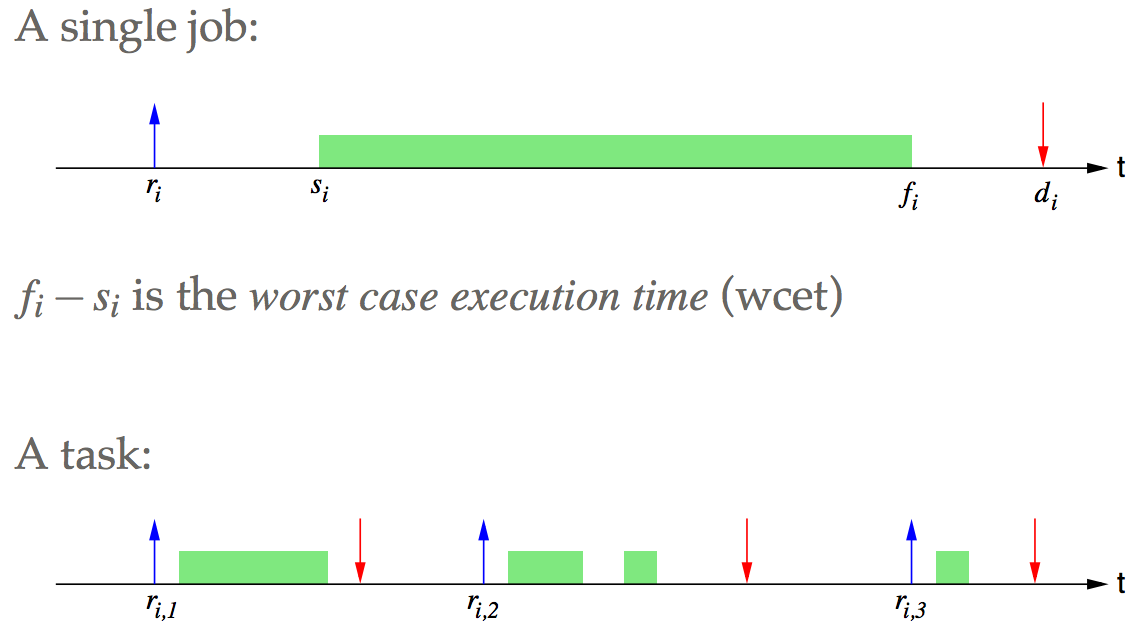
\includegraphics[scale=.5]{jobtask}
\end{figure}

\section{Scheduling}
A Scheduling algorithm is a strategy used to pick a \emph{ready} task for 
execution. There are two types:
\begin{enumerate}
  \item Preemptive: The running task can be temporarily suspended to execute 
    another task
  \item Non preemptive: The running task cannot be suspended until completion or
    until it is blocked.
\end{enumerate}
A \emph{schedule} is a particular assignment of tasks to the processor. Here is 
some important derived terminology with regard to scheduling:
\begin{itemize}
  \item Lateness: $L_{i} = f_{i} - d_{i} $ Want this to be $\leq 0$
  \item Tardiness: $max(0,L_{i})$
  \item Residual wcet: $c_{i}(t)$
  \item Slack: $d_{i} - t - c_{i}(t)$  How sloppy can I be
  \item Jitter: time variation of a periodic event
\end{itemize}

\begin{figure}[H]
  \centering
  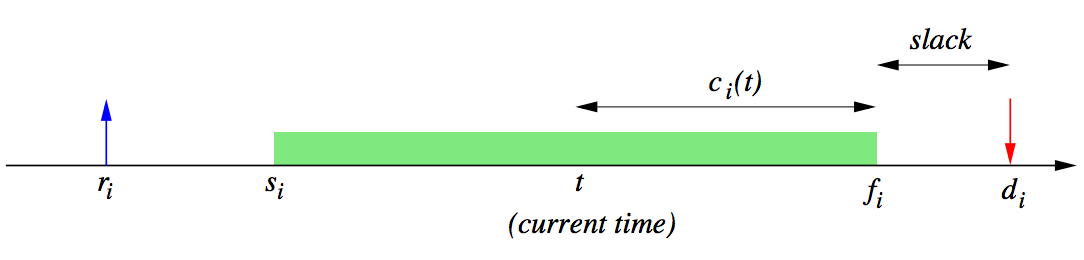
\includegraphics[scale=.6]{schedule}
\end{figure}
\begin{figure}[H]
  \centering
  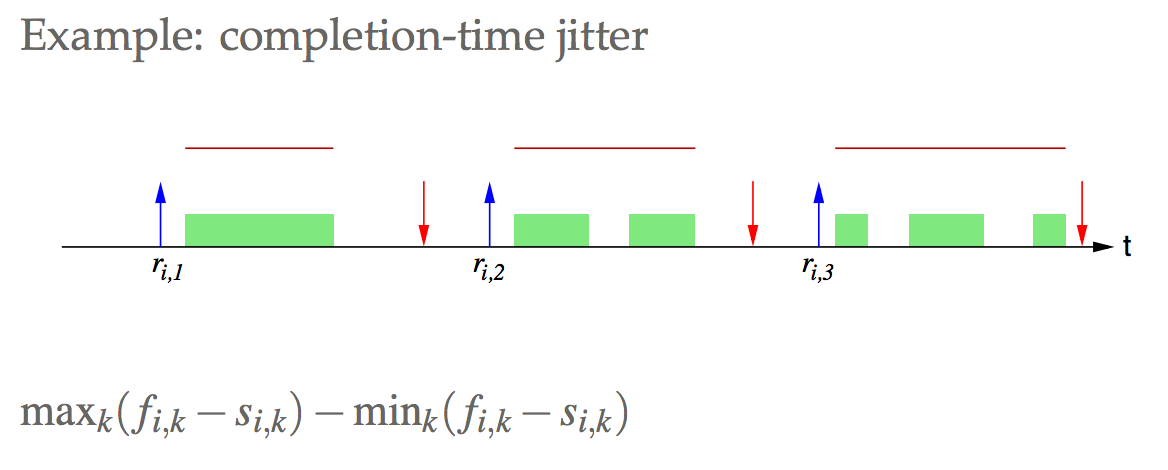
\includegraphics[scale=.6]{jitter}
\end{figure}

\subsection{Scheduling Algorithms}
A schedule is \emph{feasible} if all tasks are able to complete with
their set of constraints. A set of tasks K is set to be \emph{schedulable} if a 
feasible schedule exists. Scheduling algorithms can be:
\begin{itemize}
  \item Preemptive or non-preemptive
  \item Static or Dynamic: are the scheduling decisions based on parameters that
    change with time? For static, the parameters for all processes needed for the
    schedule are known before hand.
  \item Online or Offline: are the decisions made prior with knowledge of task 
    activations, or are they taken at run time based on the set of active tasks?
    These are different from Static/Dynamic in the sense that they describe when
    you are going to run the algorithm for scheduling. 
  \item Optimal or heuristic: can you prove that the algorithm optimizes a 
    certain criteria or not?
\end{itemize}
Optimality simply means are we trying to minimize or maximize some parameter. 
For example, minimizing the maximum lateness, minimizing the number of missed 
deadlines, or maximize the value of of feasible tasks given than tasks are 
assigned some utility value.

\subsection{Resource Constraints}
Resources (locks) can often be limited or even unavailable. Shared resources 
often require mutual exclusion. Both of these concepts lead to delays. Therefore
simply have a \emph{faster} processor doesn't always mean it is easier to meed
deadlines:
\begin{figure}[H]
  \centering
  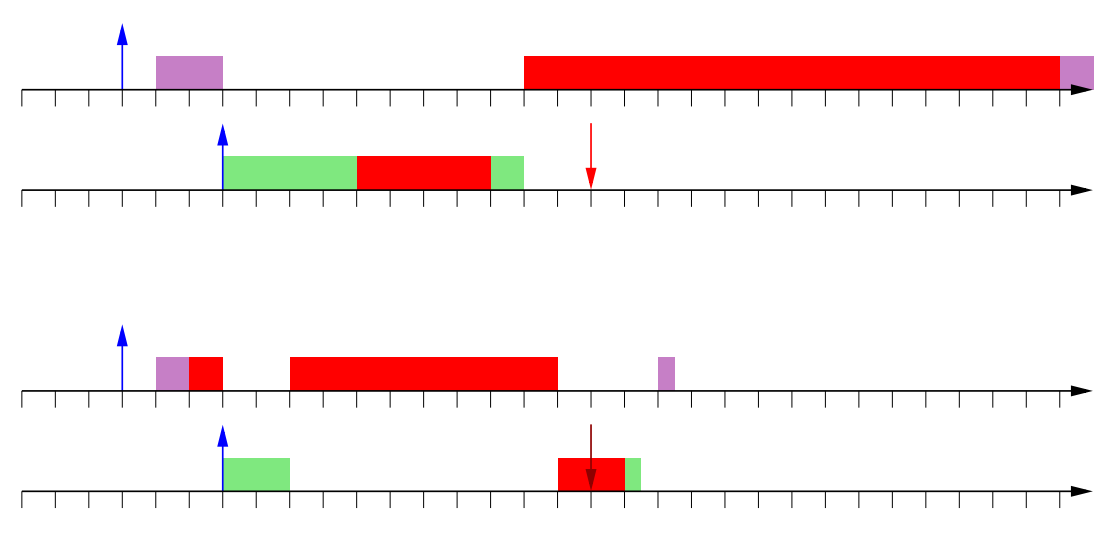
\includegraphics[scale=.6]{faster}
\end{figure}

\subsection{First Come Fist Serve (FCFS)}
A simply policy in which processes are given access to the CPU in the order of 
their arrival time. However, it is very unpredictable as the response time
depends strongly on task arrivals. It is not suitable for real time systems
because it is not concerned with feasibility. It has the following properties:
\begin{figure}[H]
  \centering
  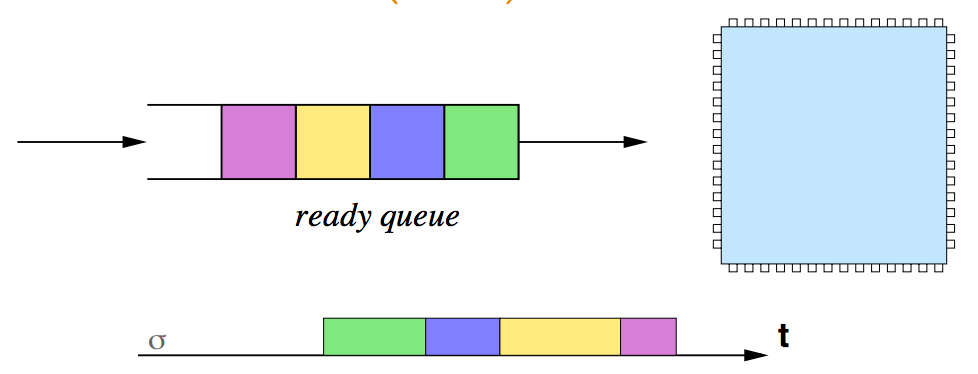
\includegraphics[scale=.5]{fcfs1}
\end{figure}

\begin{itemize}
  \item Non-preemptive
  \item Dynamic
  \item Online
  \item Heuristic
\end{itemize}

\begin{figure}[H]
  \centering
  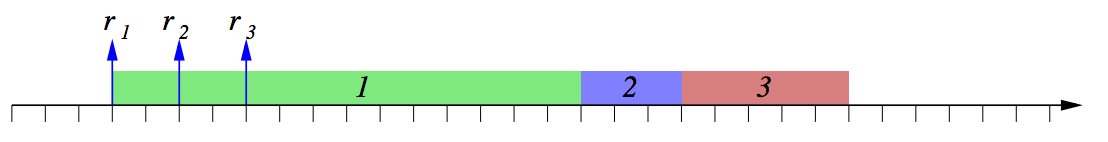
\includegraphics[scale=.6]{fcfs2}
\end{figure}

\subsection{Shortest Job First (SJF)}
This policy picks the next task with the shortest computation time. The goal of 
this algorithm is to minimize the \emph{average response time}. It also has the
following properties:
\begin{itemize}
  \item Non preemptive or preemptive
  \item Static ($c_{i}$ is known and fixed)
  \item Online or offline
  \item Optimal: It minimizes the average response time
\end{itemize}

\begin{figure}[H]
  \centering
  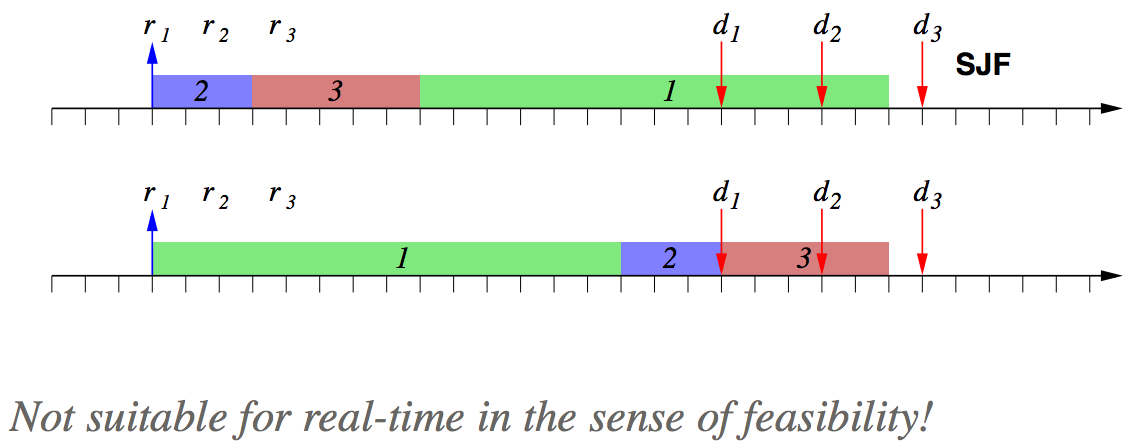
\includegraphics[scale=.6]{sjf}
\end{figure}

\subsubsection{Proof for SJF}
The following proof is not rigorous but will suffice for the purposes of this
class. \\

To prove SJF we will use a simple interchange argument. We start with a
schedule $\sigma$ where $\sigma = {j_1, j_2 \dots j_k \dots j_n}.$ In this
schedule $\sigma$ we have two jobs $j_i$ and $j_k$ such that $c_i \leq c_k$.
Now lets assume that the schedule $\sigma$ is such that $\sigma = {j_1, j_2
\dots j_{i-1}, j_k, j_{i+1} \dots j_{k-1}, j_l, j_{k+1} \dots j_n}$. We must
  show that if we interchange the positions of $j_i$ and $j_k$ to produce a
  schedule $\sigma '$ that the new schedule $\sigma '$ has at least as good an
  average response time as $\sigma$. If we look at both schedule $\sigma$ and
  $\sigma$ we first realize that the average response time between $j_1 \dots
  j_{i-1}$ and $j_{k+1} \dots j_n$ in both schedules is equal. For the jobs
  $j_i \dots j_k$ in $\sigma '$ and $j_k, j_{i+1} \dots j_{k-1}, j_i$ we every
  job in $\sigma '$ will have a lower resposne time since $c_i \leq c_k$ and
  every job after the first one in $\sigma '$ (for this subset of jobs) will
  finish earlier than the corresponding job in $\sigma$. Thus, we can conclude
  that the average resposne time for this subset of jobs is less than or equal
  in $\sigma '$ than in $\sigma$. Consequently, the average response time in
  $\sigma '$ is less than equal to that of $\sigma$. If we make a finite number
  of such transpositions, we can see that $\sigma_{SJF}$ will minimize average
  response time.


\subsection{Priority Scheduling}
Each task is assigned a priority $p_{i}$ and the task with the highest priority
is selected first. Tasks with the same priority are scheduling using FCFS. It has
the following properties:
\begin{itemize}
  \item Preemptive
  \item Static or Dynamic based on how you define priority
  \item Online
  \item Optimal
\end{itemize}
A common issue that pops up is \emph{Starvation:} low priority tasks may 
experience long delays due to preemption by higher priority tasks. This is 
commonly resolved by \emph{Aging:} the priority of tasks increases with waiting
time.

A few things to note with regards to defining priority:
\begin{itemize}
  \item If $p_{i} = 1/c_{i}$: shortest job first!
  \item If $p_{i} = const$: first come first served!
\end{itemize}

\subsection{Round Robin (RR)}
There is a ready queue which follows FCFS. However, each task cannot execute more
than $Q$ time units. When $Q$ time units have elapsed, the task is put back into 
the ready queue. It has to following properties:
\begin{itemize}
  \item Preemptive
  \item Dynamic
  \item Online
  \item Heuristic
  \item For very small $Q$: Each task runs as if it were executing on a virtual 
    processor that is $n$(number processes) times slower than real one
  \item For very large $Q$: RR $=$ FCFS when $Q \geq C_{i}$
\end{itemize}

\begin{figure}[H]
  \centering
  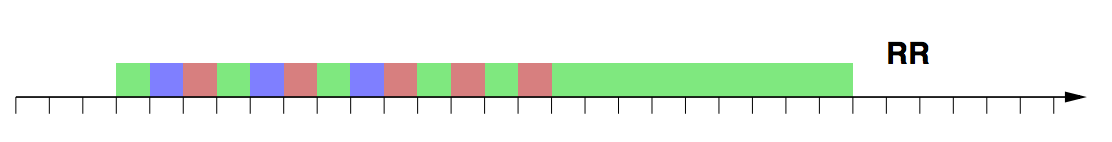
\includegraphics[scale=.6]{rr}
\end{figure}


\section{Aperiodic Real\-Time Scheduling}
There are three main types of tasks we are concerned about:
\begin{enumerate}
  \item \emph{System Tasks:} Each task has a priority and is usually preemptive.
    This are the most important tasks and usually have a dedicated system 
    priority queue.
  \item \emph{Interactive Tasks:} These are tasks such as commands run on the 
    command line. We use RR to maintain fairness and the response time is 
    proportional to the load (medium priority).
  \item \emph{Batch Task:} These tasks are run when there is free time to run 
    them later and the output is redirected to some file to be read later. These
    are lowest priority. $P_{i} = 1/r_{i}$
\end{enumerate}
\begin{figure}[H]
  \centering
  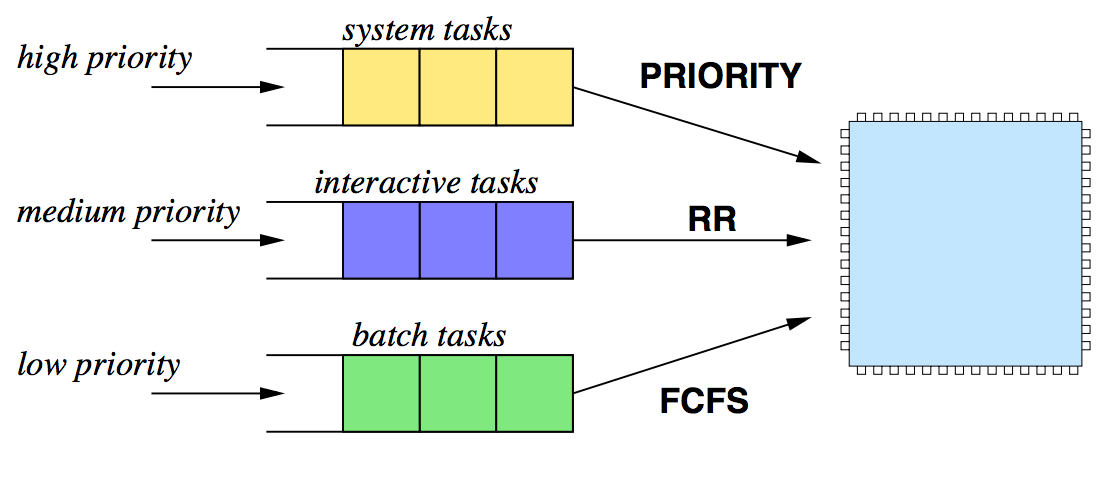
\includegraphics[scale=.6]{tasks}
\end{figure}

\subsection{Earliest Due Date (EDD)}
The algorithm selects the task with the earliest \emph{relative} deadline. All
the tasks arrive simultaneously and have a fixed known priority $D_{i}$. 
Preemption is not an issue and the goal is to \emph{minimize the maximum 
lateness $L_{max}$}. EDD guarantees a feasible (every task will meet its deadline)
schedule as long as feasible schedule exists. The priority of a task will be 
$1/D_{i}$
\begin{itemize}
  \item Non-preemptive
  \item Static
  \item Offline
  \item Optimal - minimize max lateness
\end{itemize}

\begin{figure}[H]
  \centering
  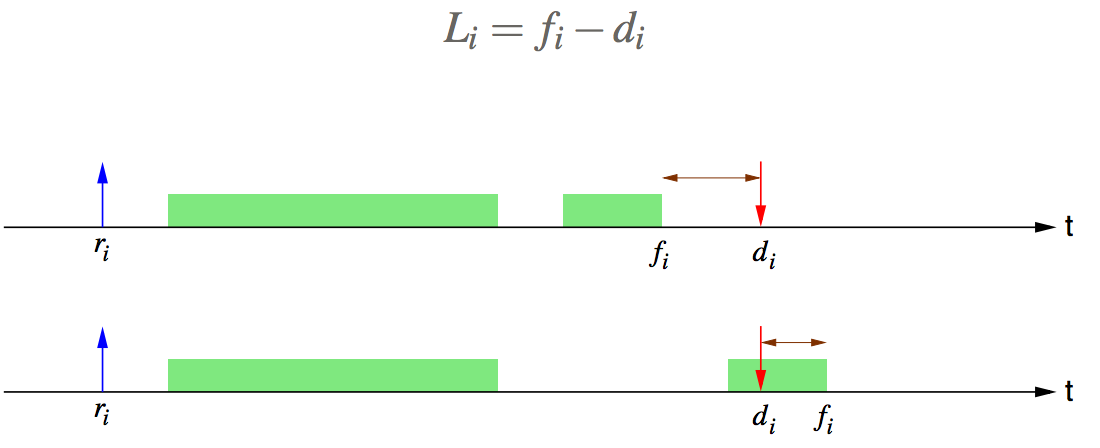
\includegraphics[scale=.6]{edd}
\end{figure}
\begin{figure}[H]
  \centering
  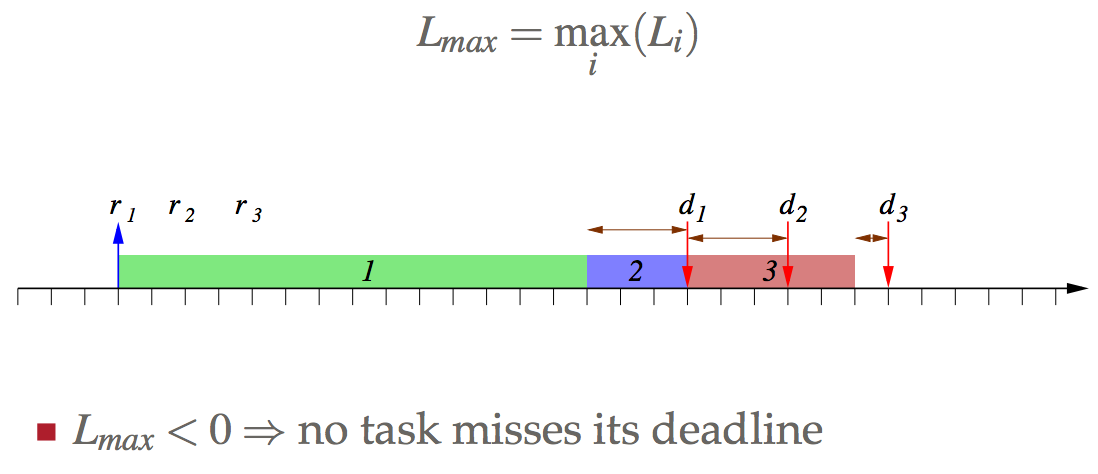
\includegraphics[scale=.6]{edd2}
\end{figure}
EDD can be proved using \emph{Jackson's Rule:} Given a set of n independent tasks
,any algorithm that executes the tasks in order of increasing deadlines is optimal
with respect to maximum lateness.

\subsubsection{Proof for EDD}
The following proof is not a completely rigorous attempt at proving EDD but
will suffice for the purposes of this class. First we realize that we are
essentially trying to prove \textbf{Jackson's Rule}. \\

\textbf{Theorem (Jackson's Rule)} : \textit{Given a set of n independent tasks,
any algorithm that executes the tasks in the order of non-decreasing deadlines
is optimal with respect to maximum lateness} \\

\textbf{Proof} To prove Jackson's theorem we will use an interchange argument.
Let $\sigma$ be a schedule produced by any algorithm $A$. If $A$ is not the
same as EDD then, there are two jobs $J_a$ and $J_b$ such that $d_a \leq d_b$
where $J_b$ immediately precdes $J_a$ in the schedule $\sigma$. Lets switch
$J_b$ and $J_a$ to produce a new schedule $\sigma '$. In $\sigma '$, $J_a$
immediately precedes $J_b$. These two schedules are shown in the figure
\figref{jackson}. \\

From figure \figref{jackson} we can see that for $\sigma$ the maximum lateness is
$f_a - d_a$. Lets compare this with the maximum lateness of $\sigma '$. Here we
have two cases :

\begin{enumerate}
  \item $L'_a \geq L'_b$ Then we know that the maximum lateness between $J_a$
    and $J_b$ in $\sigma '$ is less than or equal to$f_a - d_a$ and thus the
    maximum lateness of $\sigma '$ is less than or equal to that of $\sigma$.
  \item $L'_b \geq L'_a$ Then we know that $f'_b = f_a$ and thus since $d_b
    \geq d_a$, $L'b \leq L_a$. That is, $f'_b - d_b \leq f_a - d_a$ and thus
    the maximum lateness of $\sigma '$ is less than or equal to the maximum
    latness of $\sigma$.
\end{enumerate}

From both cases we can see that by interchanging $J_b$ and $J_a$ the maximum
lateness is at least as good as it was before the interchanging. Thus we can
conclude that interchanging $J_b$ and $J_a$ does not increase maximum lateness
and a finite number such such transpositions can transpose $\sigma$ into an EDD
schedule which in turn will have minimum maximum latness. 
\begin{figure}[H]
  \centering
  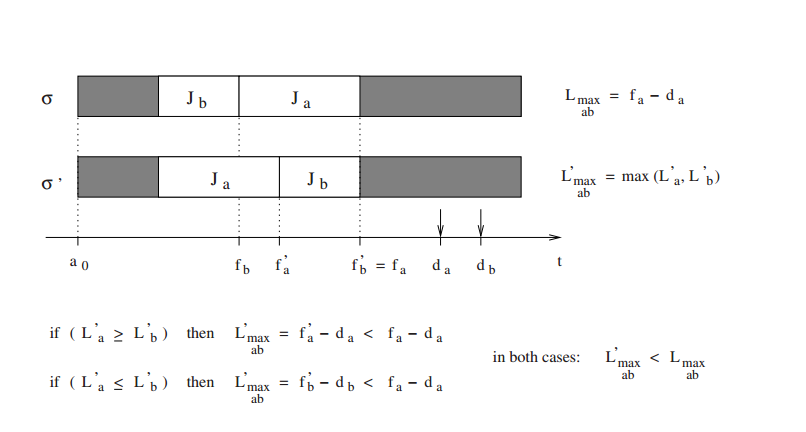
\includegraphics[scale=0.75]{jacksons}
  \label{fig:jackson}
\end{figure}


\subsection{Earliest Deadline First (EDF)}
The algorithm selects the task with the earliest \emph{absolute} deadline. Tasks
can arrive anytime and have a dynamic priority $d_{i}$ depending on when the 
tasks arrive. The tasks are preemptive and the goal is to again \emph{minimize 
the maximum lateness $L_{max}$}. Under non-preemptive scheduling, EDF, is not
optimal and cannot produce a feasible schedule.
\begin{itemize}
  \item Preemptive
  \item Dynamic
  \item Online
  \item Optimal - minimize max lateness
\end{itemize}
\begin{figure}[H]
  \centering
  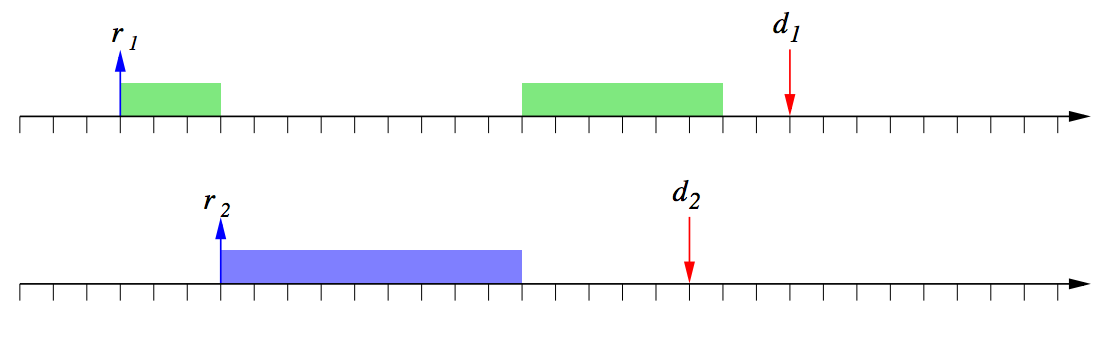
\includegraphics[scale=.6]{edf}
\end{figure}


\section{Periodic Real\-Time Scheduling}
Period tasks are those that have jobs that repeat at a regular interval in time.
\begin{figure}[H]
  \centering
  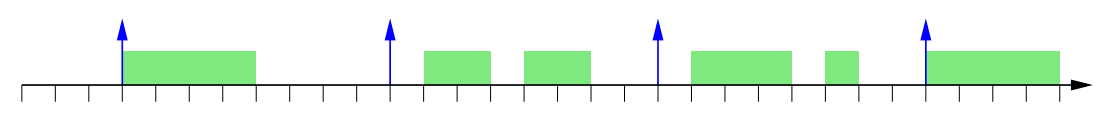
\includegraphics[scale=.6]{period}
\end{figure}

\subsection{Timeline Scheduling}
A classic technique in which the time axis is divided into intervals of equal 
length (slots). Each task is \emph{statically} allocated in order to meet
desired request rate. Timers are used to activate execution in each slot.
\begin{itemize}
  \item Minor Cycle: GCD of periods - it tells you when you need to make 
    decisions on what to run or context switching.
  \item Major Cycle: LCM of periods - it tells you when the whole cycle repeats
    and how big a program would be.
\end{itemize}
\begin{figure}[H]
  \centering
  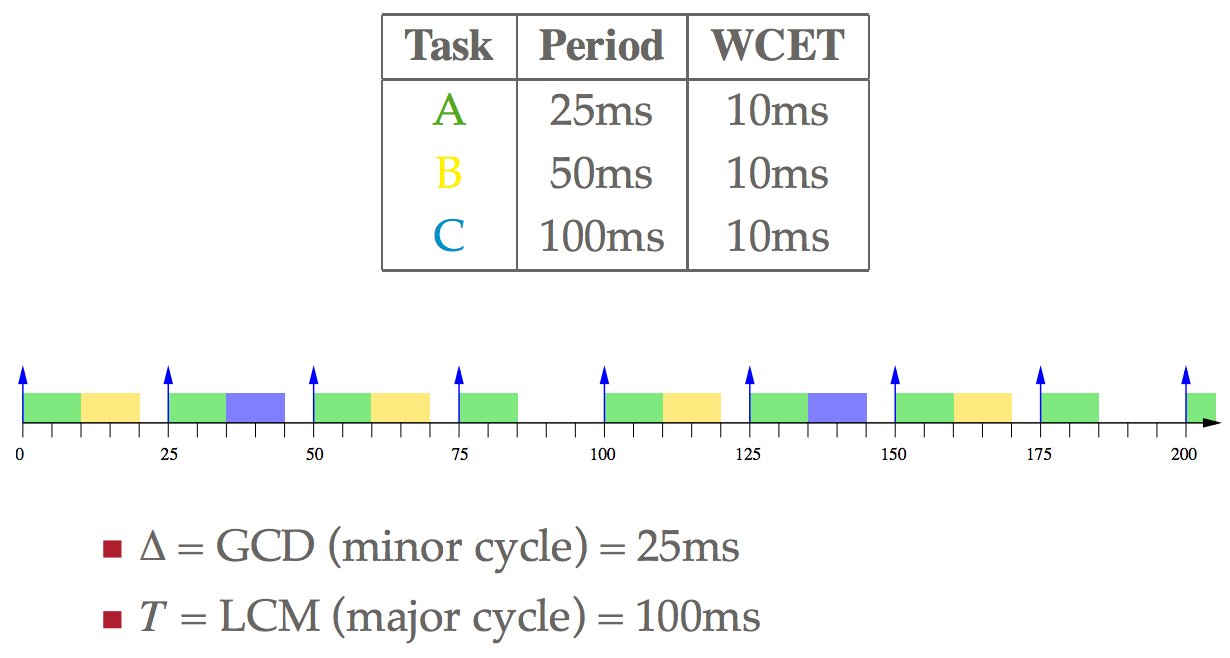
\includegraphics[scale=.6]{timeline}
\end{figure}
Advantages:
\begin{itemize}
  \item Simple implementation
  \item Low run-time overhead
  \item Jitter can be controlled
\end{itemize}
Disadvantages:
\begin{itemize}
  \item Not robust to overloads/overruns
  \item Difficult to expand the schedule
  \item Not easy to handle aperiodic activities
\end{itemize}
If the schedule becomes overloaded, a task might not meet its deadline and there
can be a domino effect. If the task is aborted, the system could be in an 
inconsistent state (undefined). If a certain task is updated and now takes more
time, you may have to re-do the entire schedule. A common approach to this 
problem is to split the task into two sub tasks and then re-build the schedule.

\subsection{Rate Monotonic Scheduling}
Each task in assigned a fixed priority proportional to its rate. The big question
here is how can we determine feasibility?
\begin{itemize}
  \item Each task uses the processor for a fraction of time: $U_{i} = C_{i}/T_{i}$
  \item The total processor utilization is: $U_{cpu} = \sum\limits_{i} U_{i}$
  \item $U_{cpu}$ measures the processor load. If $U_{cpu} > 1$, the processor
    is overloaded so the task set cannot be scheduled. 
  \item Liu: For $n$ periodic tasks if $U_{cpu} \leq n(2^{1/n}-1)$, then RM will
    produce a feasible schedule. In the limit $n \rightarrow \infty$, RHS is 
    $ln(2)$
\end{itemize}
\begin{figure}[H]
  \centering
  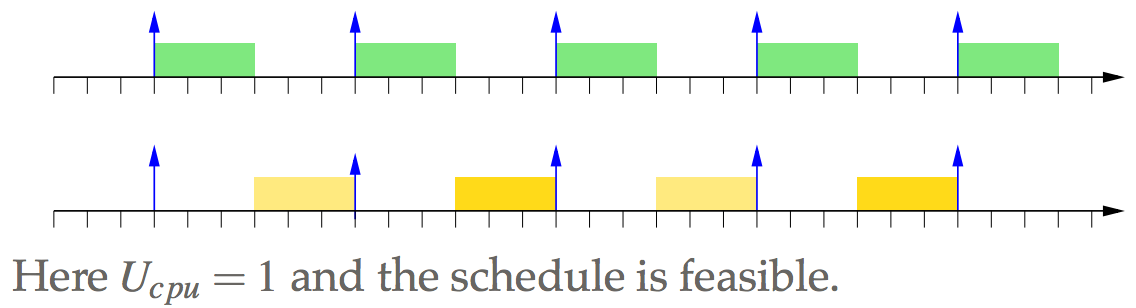
\includegraphics[scale=.6]{rm}
\end{figure}

\section{Priority Inheritance}
Priority Inversion is a problem in which a high priority task is indirectly 
preempted by a medium priority task effectively `inverting' the relative 
priorities of the two tasks for an unbounded interval of time. To mitigate, 
this problem, there are four protocols presented below.

\subsection{Non-Preemptive Protocol}
Preemption is forbidden in Critical Sections. To implement this: when a task 
enters a critical section, increase its priority to max of all the other 
processes priorities. The problem with this design is that high priority tasks
that do not interfere with the CS will be blocked.
\begin{figure}[H]
  \centering
  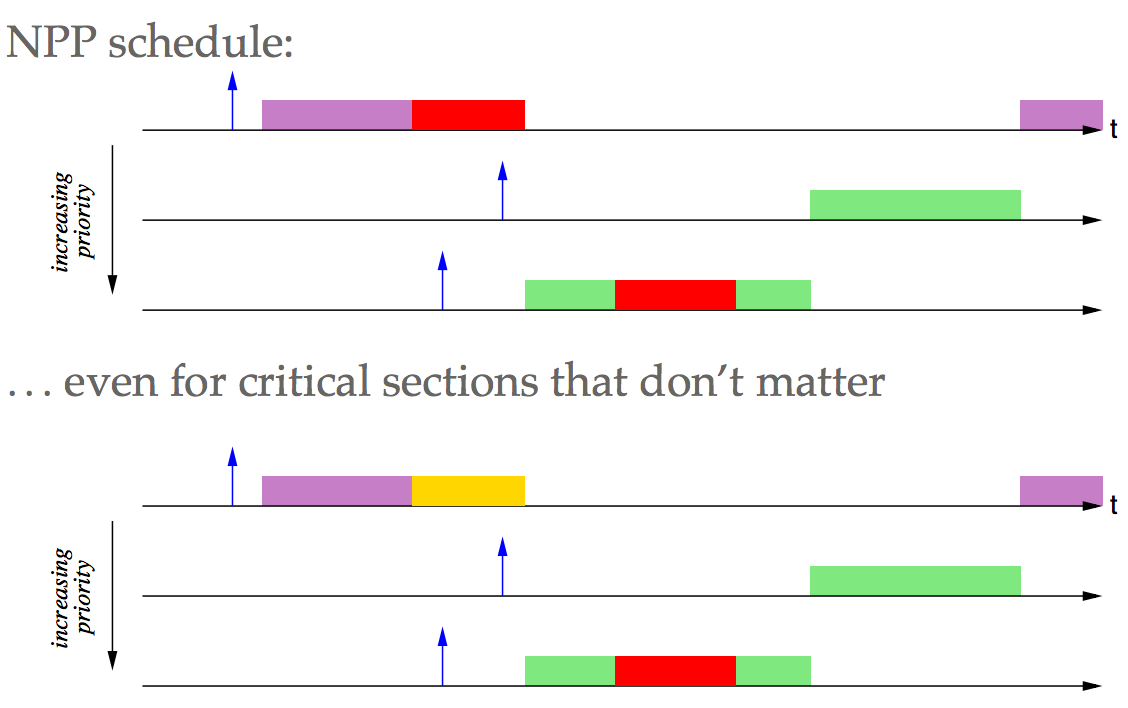
\includegraphics[scale=.6]{npp}
\end{figure}

\subsection{Highest Locker Priority}
A task in the critical section gets the highest priority among the tasks that 
use the CS. To implement: when a task enters a CS, increase its priority to the
max value of the tasks that may access the same critical section. A process 
could be blocked because it \emph{might} enter the critical section, not because
it is in the critical section.
\begin{figure}[H]
  \centering
  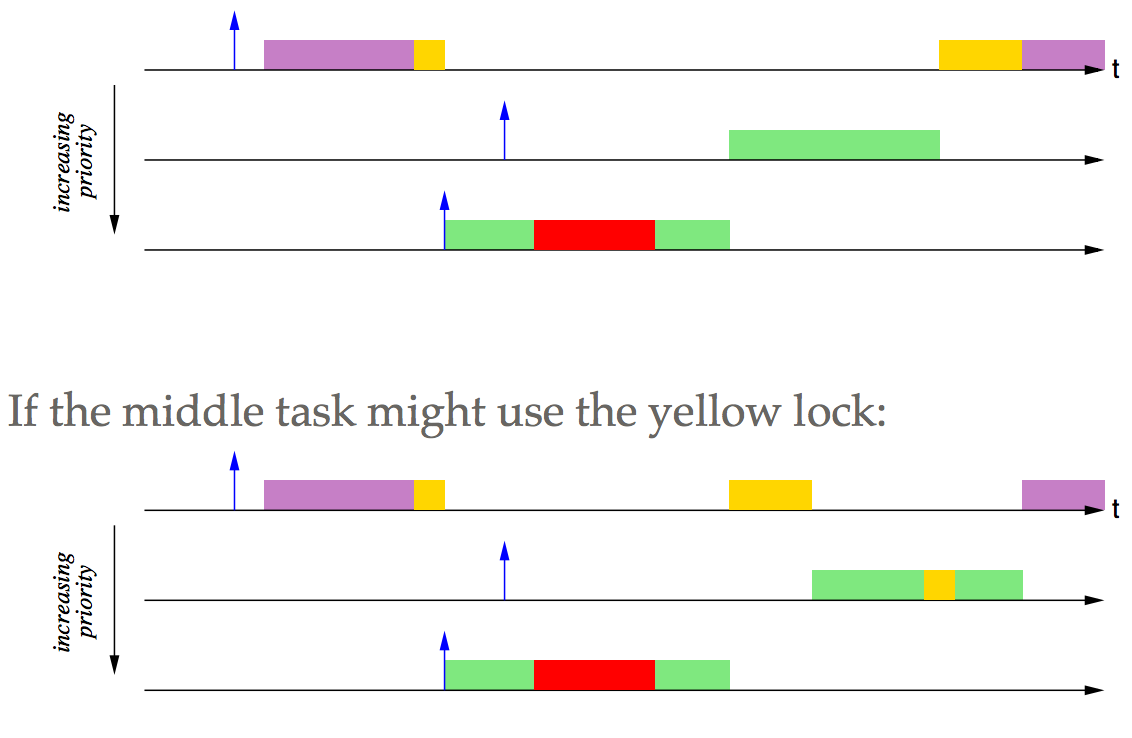
\includegraphics[scale=.6]{hlp}
\end{figure}

\subsection{Priority Inheritance Protocol}
A task in a critical section increases its priority only if it blocks other 
tasks. A task in a critical section inherits the highest priority among those 
tasks that it blocks. There are two types of blocking:
\begin{enumerate}
  \item Direct: task blocked on a lock
  \item Push-through: task blocked because a lower priority task inherited a 
    higher priority (indirectly)
\end{enumerate}
\begin{figure}[H]
  \centering
  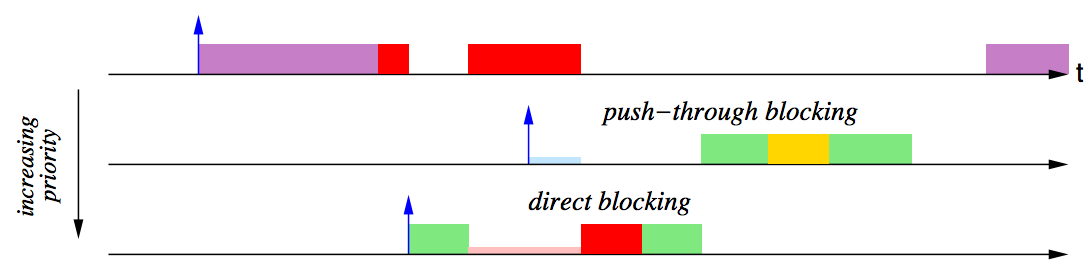
\includegraphics[scale=.6]{pip1}
\end{figure}
\begin{figure}[H]
  \centering
  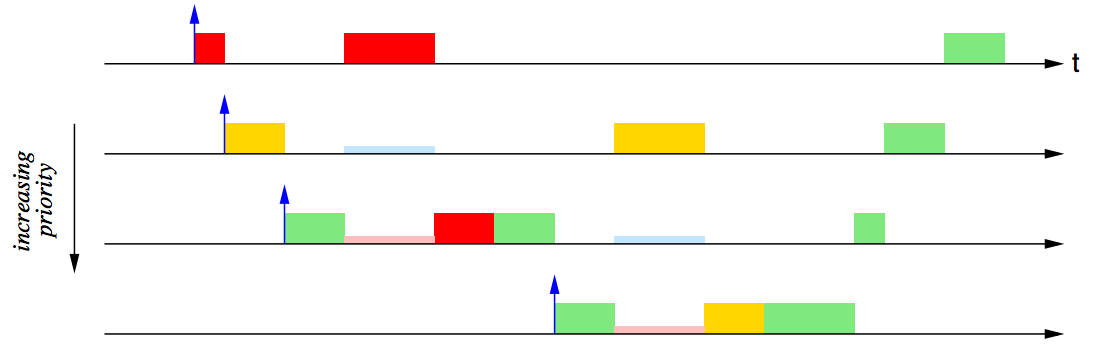
\includegraphics[scale=.6]{pip2}
\end{figure}
Problem: \emph{Chained Blocking:} higher priority processes get constantly 
blocked while waiting for lower priority processes to finish CS.
\begin{figure}[H]
  \centering
  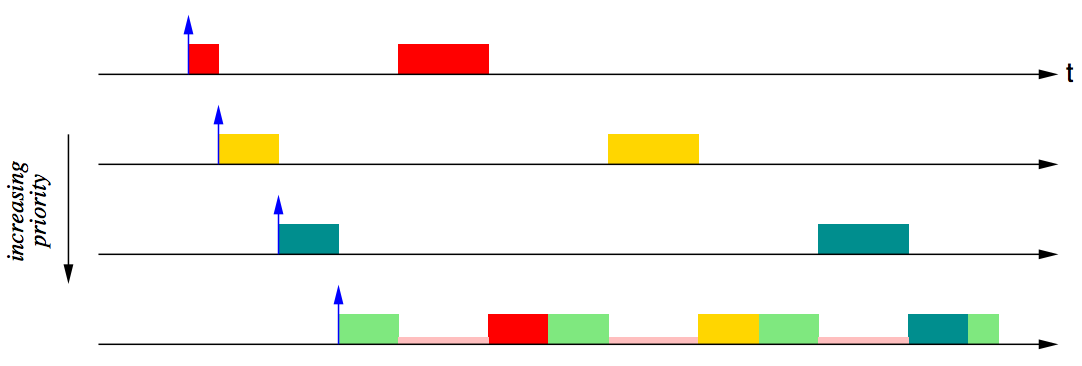
\includegraphics[scale=.6]{pip3}
\end{figure}

\subsection{Priority Ceiling Protocol}
This algorithm aims to reduce chained blocking and is a modification to the PIP
protocol. Each semaphore is assigned a priority ceiling equal to
the highest priority of the tasks that can lock it. Then, a task $T_{i}$ is 
allowed to enter a critical section only if its priority is higher than all 
priority ceilings of the semaphores currently locked by tasks. If you are inside
a CS and end up blocking a task, you inherit the priority of the task that you 
blocked until you relinquish the CS that gave you that authority.
$T_{i}$.
\begin{figure}[H]
  \centering
  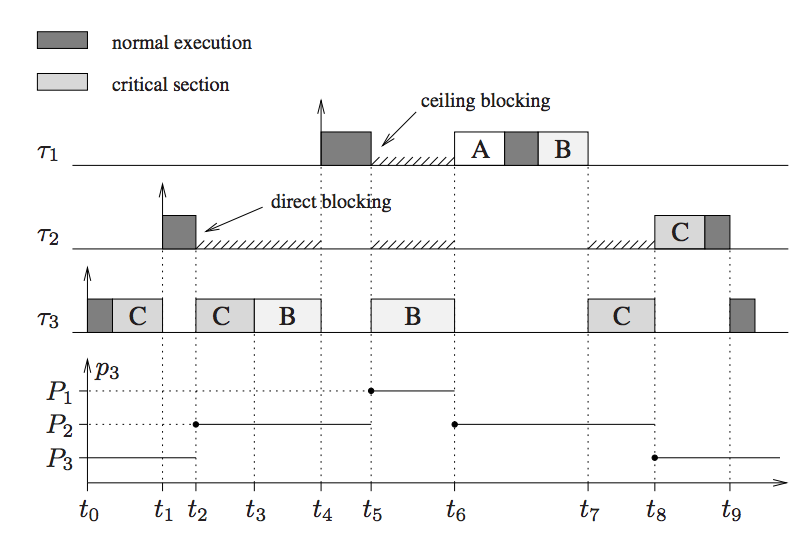
\includegraphics[scale=.7]{pcp}
\end{figure}


\section{Communication Protocols}
With regard to what we previously talked about with Daisy Chaining, devices
can send signals to the CPU. However, we have not yet discussed how the 
signals are transmitted between the wires. Here is some vocabulary:
\begin{itemize}
  \item Synchronous: Having one line for data and a separate line for clock to
    keep track of when a bit is sent or received. 
  \item Parity: Way to check for error, it is the XOR of all the bits
    \subitem Even: xor of bits = 0
    \subitem Odd: xor of bits = 1
    \subitem Error checking is very weak bc can only check for 1 bit of error
  \item Baud Rate: frequency of you are transmitting/receiving at
  \item Flow Control: method of tell tranismitter to Stop/Start. It is used if 
    you have error or if using a finite buffering system.
\end{itemize}

\subsection{RS-232}
This is a very simple and resilient protocol that was used initially to connect
to a modem.
\begin{figure}[H]
  \centering
  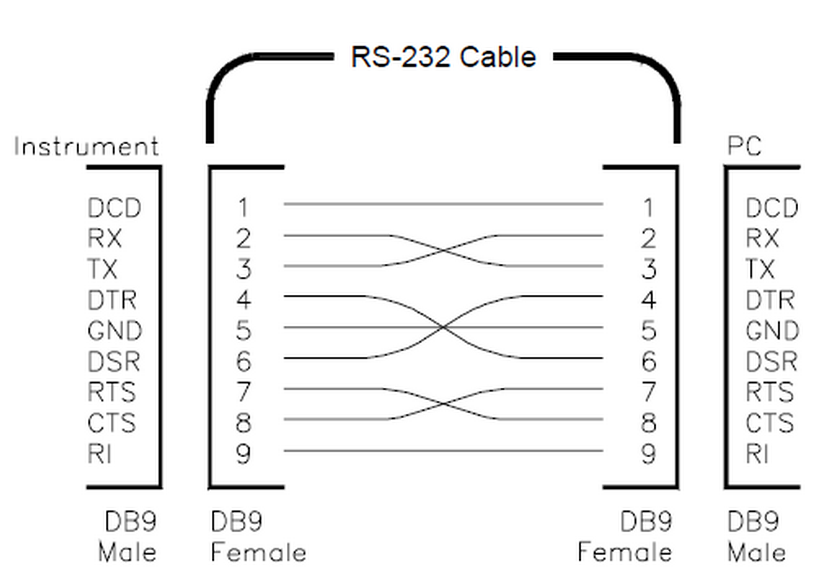
\includegraphics[scale=.6]{rs1}
\end{figure}

\begin{itemize}
  \item Large voltage swings to amplify signal to noise ratio (1:-12V 0:+12V)
  \item Can be half duplex (1 comm direction at a time) or full duplex
  \item Asynchronous 
  \item Limited to 7-8 bits at a time per transmission for data and 0-1 parity 
    bits per transmission.
    \subitem 8 bits are are communicating bytes. 7 bits are used for communicating
    ASCII
  \item Both transmiter and receiver have to agree on how many bits sent, what
    type of parity, and baud rate before communicating.
  \item Advantages: Simple, resilient to noise, can transmit over long distances
  \item Disadvantages: Slow b/c there is no internal clock, drains power
  \item Software Flow Control: XON/XOFF (17)/(19)
  \item Hardware Flow Control: RTS/CTS - assigned bits on the serial port
\end{itemize}
\begin{figure}[H]
  \centering
  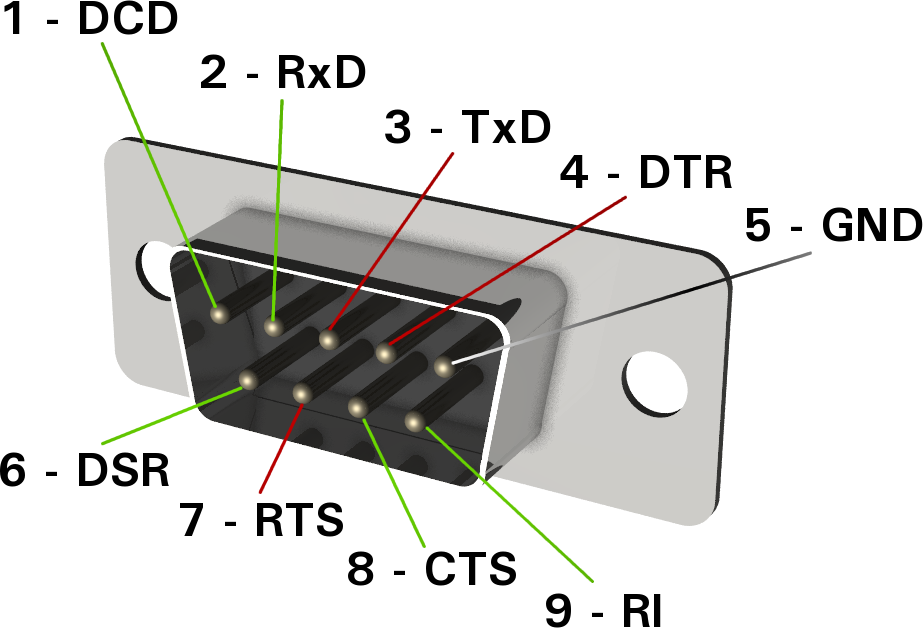
\includegraphics[scale=.25]{rs2}
\end{figure}
\begin{figure}[H]
  \centering
  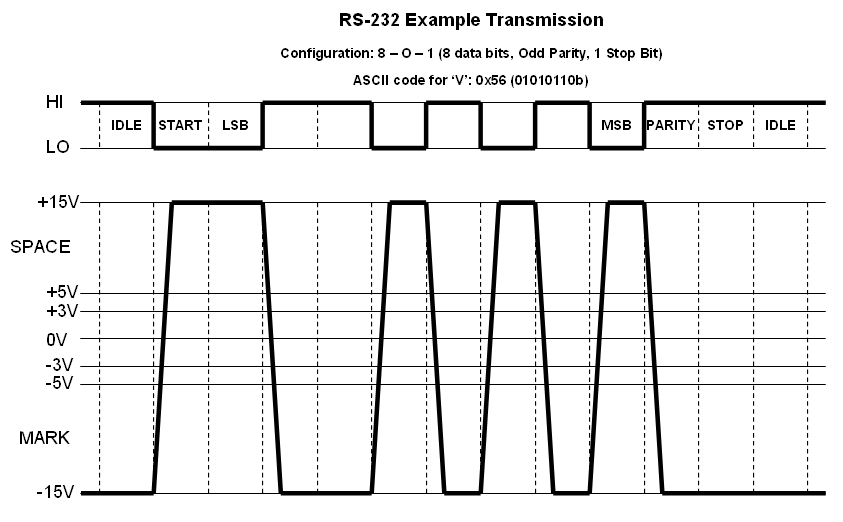
\includegraphics[scale=.4]{rs3}
\end{figure}


\end{document}

